\chapter{Arhitektura i dizajn sustava}
%		
%		\textbf{\textit{dio 1. revizije}}\\
%
%		\textit{ Potrebno je opisati stil arhitekture te identificirati: podsustave, preslikavanje na radnu platformu, spremišta podataka, mrežne protokole, globalni upravljački tok i sklopovsko-programske zahtjeve. Po točkama razraditi i popratiti odgovarajućim skicama:}
%	\begin{itemize}
%		\item 	\textit{izbor arhitekture temeljem principa oblikovanja pokazanih na predavanjima (objasniti zašto ste baš odabrali takvu arhitekturu)}
%		\item 	\textit{organizaciju sustava s najviše razine apstrakcije (npr. klijent-poslužitelj, baza podataka, datotečni sustav, grafičko sučelje)}
%		\item 	\textit{organizaciju aplikacije (npr. slojevi frontend i backend, MVC arhitektura) }		
%	\end{itemize}

		

				
		\section{Baza podataka}
			
			Podatci potrebni za funkcioniranje naše aplikacije pohranjuju se u relacijsku bazu podataka. Osnovni objekt relacijske baze podataka je relacija - imenovana dvodimenzionalna tablica čiji stupci predstavljaju atribute, a retci opisuju entitete baze podataka (retci u relaciji zovu se n-torke).
			Sljedeći entiteti sačinjavaju bazu podataka naše aplikacije:
			\begin{packed_item}
				\item Igrač (\textit{player})
				\item Kartograf (\textit{mapper})
				\item Administrator (\textit{admin})
				\item Borba (\textit{fight})
				\item Lokacija (\textit{location})
				\item Kategorija lokacije (\textit{category})
				\item Karta (\textit{card})
				\item Špil karata (\textit{deck})
			\end{packed_item}
			
			\subsection{Opis tablica}
			
				\noindent\textbf{player} $($Igrač$)$ - Ovaj entitet sadržava podatke o korisniku. Svaki korisnik je ujedno i igrač. Sadrži atribute: korisničko ime, lozinku, e-mail adresu, fotografiju i bodove igrača. Ovaj entitet je u \textit{One-to-Many} vezi s entitetom card preko atributa username i ima dvije \textit{One-to-Many} veze s entitetom fight, koje se odnose na borbe u kojima je igrač pobijedio i borbe u kojima je izgubio. 
				
				\begin{longtabu} to \textwidth {|X[7, l]|X[6, l]|X[20, l]|}
					
					\hline \multicolumn{3}{|c|}{\textbf{player}}	 \\[3pt] \hline
					\endfirsthead
					
					\hline \multicolumn{3}{|c|}{\textbf{player}}	 \\[3pt] \hline
					\endhead
					
					\hline 
					\endlastfoot
					
					\cellcolor{LightGreen}username & VARCHAR(15) 	&  	jedinstveni identifikator korisnika 	\\ \hline
					password\_hash & VARCHAR(20)  &   hash lozinke \\ \hline 
					email & VARCHAR(20)  &   e-mail adresa korisnika \\ \hline 
					photo & UUID & fotografija (avatar$)$ korisnika \\ \hline 
					points & INT	&  	broj bodova igrača	\\ \hline 
					
				\end{longtabu}
				
				\noindent\textbf{mapper} $($Kartograf$)$ - Entitet mapper nasljeđuje entitet player. Ovaj entitet, uz atribute playera, ima i atribute IBAN i ID photo.
				
				\begin{longtabu} to \textwidth {|X[7, l]|X[6, l]|X[20, l]|}
					
					\hline \multicolumn{3}{|c|}{\textbf{mapper}}	 \\[3pt] \hline
					\endfirsthead
					
					\hline \multicolumn{3}{|c|}{\textbf{mapper}}	 \\[3pt] \hline
					\endhead
					
					\hline 
					\endlastfoot
					
					\cellcolor{LightGreen}username & VARCHAR(15) 	&  	jedinstveni identifikator korisnika 	\\ \hline
					password\_hash & VARCHAR(20)  &   hash lozinke \\ \hline 
					email & VARCHAR(20)  &   e-mail adresa korisnika \\ \hline 
					photo & UUID & fotografija (avatar$)$ korisnika \\ \hline 
					points & INT	&  	broj bodova igrača	\\ \hline 
					iban & VARCHAR(21)  & IBAN računa za uplatu plaće \\ \hline 
					id\_photo & UUID & fotografija osobne iskaznice \\ \hline 
					
				\end{longtabu}
			
				\noindent\textbf{admin} $($Administrator$)$ - Entitet admin nasljeđuje entitet player. Ovaj entitet ima iste atribute kao i entitet player.
				
				\begin{longtabu} to \textwidth {|X[7, l]|X[7, l]|X[20, l]|}
					
					\hline \multicolumn{3}{|c|}{\textbf{admin}}	 \\[3pt] \hline
					\endfirsthead
					
					\hline \multicolumn{3}{|c|}{\textbf{admin}}	 \\[3pt] \hline
					\endhead
					
					\hline 
					\endlastfoot
					
					\cellcolor{LightGreen}username & VARCHAR(15)	&  	jedinstveni identifikator korisnika 	\\ \hline
					password\_hash & VARCHAR(20) &   hash lozinke \\ \hline 
					email & VARCHAR(20) &   e-mail adresa korisnika \\ \hline 
					photo & UUID & fotografija (avatar$)$ korisnika \\ \hline 
					points & INT	&  	broj bodova igrača	\\ \hline 
					
				\end{longtabu}
			
				\noindent\textbf{fight} $($Borba$)$ - Ovaj entitet sadržava podatke o održanim borbama između igrača. Sadrži atribute: ID borbe, trenutak početka borbe, vrijeme trajanja borbe, korisničko ime igrača koji je pobijedio i korisničko ime igrača koji je izgubio. Ovaj entitet ima dvije \textit{Many-to-One} veze s entitetom player preko korisničkih imena pobjednika i gubitnika.
				
				\begin{longtabu} to \textwidth {|X[6, l]|X[6, l]|X[20, l]|}
					
					\hline \multicolumn{3}{|c|}{\textbf{fight}}	 \\[3pt] \hline
					\endfirsthead
					
					\hline \multicolumn{3}{|c|}{\textbf{fight}}	 \\[3pt] \hline
					\endhead
					
					\hline 
					\endlastfoot
					
					\cellcolor{LightGreen}fight\_id & INT	&  	jedinstveni brojčani identifikator borbe 	\\ \hline
					start & TIMESTAMP  &   trenutak početka borbe \\ \hline 
					duration & INTERVAL	&  	trajanje borbe	\\ \hline 
					\cellcolor{LightBlue}winner	& VARCHAR(15) & korisničko ime pobjednika borbe  	\\ \hline 
					\cellcolor{LightBlue}loser	& VARCHAR(15) & korisničko ime gubitnika borbe  	\\ \hline 
					
				\end{longtabu}

				{\noindent\textbf{location} $($Lokacija$)$ - Ovaj entitet sadržava sve važne informacije o lokacijama na kojima igrač može sakupiti karte. Sadrži atribute: ID lokacije, naziv lokacije, fotografiju lokacije i ID kategorije. Ovaj entitet u vezi je \textit{Many-to-One} s Category preko ID kategorije.}
				
				\begin{longtabu} to \textwidth {|X[6, l]|X[6, l]|X[20, l]|}
					
					\hline \multicolumn{3}{|c|}{\textbf{location}}	 \\[3pt] \hline
					\endfirsthead
					
					\hline \multicolumn{3}{|c|}{\textbf{location}}	 \\[3pt] \hline
					\endhead
					
					\hline 
					\endlastfoot
					
					\cellcolor{LightGreen}location\_id & INT	&   jedinstveni brojčani identifikator lokacije	\\ \hline
					location\_name	& VARCHAR(20) &  naziv lokacije 	\\ \hline 
					location\_photo & UUID &  fotografija lokacije \\ \hline 
					\cellcolor{LightBlue} category\_id	& INT &   jedinstveni brojčani identifikator kategorije	\\ \hline 
					
					
				\end{longtabu}
			
				{\noindent\textbf{category} $($Kategorija lokacije$)$ - Ovaj entitet sadržava sve važne informacije o kategorijama koje lokacije mogu biti. Sadrži atribute: ID kategorije, naziv kategorije i broj bodova koje kategorija nosi. Ovaj entitet u vezi je \textit{One-to-Many} s Location preko ID kategorije.}
				
				\begin{longtabu} to \textwidth {|X[6, l]|X[6, l]|X[20, l]|}
					
					\hline \multicolumn{3}{|c|}{\textbf{category}}	 \\[3pt] \hline
					\endfirsthead
					
					\hline \multicolumn{3}{|c|}{\textbf{category}}	 \\[3pt] \hline
					\endhead
					
					\hline 
					\endlastfoot
					
					\cellcolor{LightGreen}category\_id & INT	&   jedinstveni brojčani identifikator kategorije	\\ \hline
					category\_name	& VARCHAR(20) &  naziv kategorije 	\\ \hline 
					category\_points & INT &  bodovna vrijednost kategorije \\ \hline  
					
					
				\end{longtabu}
			
				{\noindent\textbf{card} $($Karta$)$ - Ovaj entitet sadržava sve važne informacije o kartama koje igrači mogu posjedovati. Sadrži atribute: ID karte, broj bodova koje karte i ID lokacije. Ovaj entitet u vezi je \textit{Many-to-One} s Location preko ID lokacije te \textit{Many-to-One} s Deck preko ID karte.}

				\begin{longtabu} to \textwidth {|X[6, l]|X[6, l]|X[20, l]|}
					
					\hline \multicolumn{3}{|c|}{\textbf{card}}	 \\[3pt] \hline
					\endfirsthead
					
					\hline \multicolumn{3}{|c|}{\textbf{card}}	 \\[3pt] \hline
					\endhead
					
					\hline 
					\endlastfoot
					
					\cellcolor{LightGreen}card\_id & INT	&   jedinstveni brojčani identifikator karte	\\ \hline 
					card\_points & INT &  bodovna vrijednost karte \\ \hline 
					\cellcolor{LightBlue} location\_id	& INT &   jedinstveni brojčani identifikator lokacije	\\ \hline 
					
					
				\end{longtabu}
			
				{\noindent\textbf{deck} $($Špil karata$)$ - Ovaj entitet sadržava sve važne informacije o špilu koje igrač posjeduje. Sadrži atribute: korisničko ime i ID karte. Ovaj entitet u vezi je \textit{One-to-One} s Player preko korisničkog imena te \textit{One-to-Many} s Deck preko ID karte.}
				
				\begin{longtabu} to \textwidth {|X[6, l]|X[6, l]|X[20, l]|}
					
					\hline \multicolumn{3}{|c|}{\textbf{deck}}	 \\[3pt] \hline
					\endfirsthead
					
					\hline \multicolumn{3}{|c|}{\textbf{deck}}	 \\[3pt] \hline
					\endhead
					
					\hline 
					\endlastfoot
					
					\cellcolor{LightBlue}username & VARCHAR(15)	&   korisničko ime igrača	\\ \hline
					\cellcolor{LightBlue} card\_id	& INT &   jedinstveni brojčani identifikator karte	\\ \hline 
					
					
				\end{longtabu}
			
			
			\subsection{Dijagram baze podataka}
				\begin{figure}[H]
					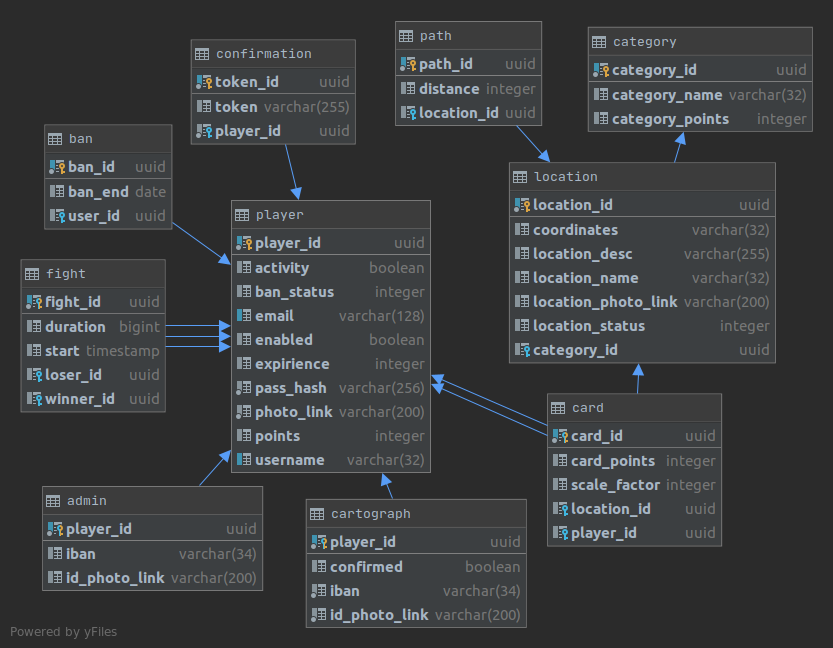
\includegraphics[width=\linewidth, height=14cm]{dijagrami/geofighterdb_diagram}				
					\centering
					\caption{E-R dijagram baze podataka}
					\label{}
				\end{figure}
			
			\eject
			
			
		\section{Dijagram razreda}
		
			\textit{Potrebno je priložiti dijagram razreda s pripadajućim opisom. Zbog preglednosti je moguće dijagram razlomiti na više njih, ali moraju biti grupirani prema sličnim razinama apstrakcije i srodnim funkcionalnostima.}\\
			
			\textbf{\textit{dio 1. revizije}}\\
			
			\textit{Prilikom prve predaje projekta, potrebno je priložiti potpuno razrađen dijagram razreda vezan uz \textbf{generičku funkcionalnost} sustava. Ostale funkcionalnosti trebaju biti idejno razrađene u dijagramu sa sljedećim komponentama: nazivi razreda, nazivi metoda i vrste pristupa metodama (npr. javni, zaštićeni), nazivi atributa razreda, veze i odnosi između razreda.}\\
			
			\textbf{\textit{dio 2. revizije}}\\			
			
			\textit{Prilikom druge predaje projekta dijagram razreda i opisi moraju odgovarati stvarnom stanju implementacije}
			
			
			
			\eject
		
%		\section{Dijagram stanja}
%			
%			
%			\textbf{\textit{dio 2. revizije}}\\
%			
%			\textit{Potrebno je priložiti dijagram stanja i opisati ga. Dovoljan je jedan dijagram stanja koji prikazuje \textbf{značajan dio funkcionalnosti} sustava. Na primjer, stanja korisničkog sučelja i tijek korištenja neke ključne funkcionalnosti jesu značajan dio sustava, a registracija i prijava nisu. }
%			
%			
%			\eject 
%		
%		\section{Dijagram aktivnosti}
%			
%			\textbf{\textit{dio 2. revizije}}\\
%			
%			 \textit{Potrebno je priložiti dijagram aktivnosti s pripadajućim opisom. Dijagram aktivnosti treba prikazivati značajan dio sustava.}
%			
%			\eject
%		\section{Dijagram komponenti}
%		
%			\textbf{\textit{dio 2. revizije}}\\
%		
%			 \textit{Potrebno je priložiti dijagram komponenti s pripadajućim opisom. Dijagram komponenti treba prikazivati strukturu cijele aplikacije.}